%!TEX root = ./binder.tex
%-------------------------------------------------------------------------------
%-------------------------------------------------------------------------------

\section{Probe Pruning}
\label{sec:probe-pruning}
%-------------------------------------------------------------------------------

We provide here the necessary background on the probe pruning techniques implemented in {\bcov} based on Agrawal~\cite{Agrawal1994}. 
The original work considered source-level pruning but only for C programs.

Given a function $F$ with a set of basic blocks $B$ connected in a CFG. 
The straightforward way to obtain complete coverage data is to probe every basic block $bb \in B$. 
However, it is possible to significantly reduce the number of required probes by computing \textit{dominance} relationships between basic blocks in a CFG. 
We say that $bb_i$ predominates $bb_j$, $bb_i\xrightharpoondown{pre}bb_j $, iff every path from function entry ($EN$) to $bb_j$ goes through $bb_i$.
Similarly, $bb_i$ postdominates $bb_j$, $bb_i\xrightharpoondown{post}bb_j $, iff every path from $bb_j$ to function exit ($EX$) goes through $bb_i$. 
We say that $bb_i$ dominates $bb_j$ iff \mbox{$bb_i\xrightharpoondown{pre}bb_j \vee bb_i\xrightharpoondown{post}bb_j $}. 
The predominator and postdominator relationships are represented by the trees $T_{pre} $ and $T_{post} $ respectively. 
The dominator graph (DG) is a directed graph that captures all dominance relationships. 
It is obtained by the union of both trees  $DG = T_{pre} \cup T_{post} $, i.e,  by merging edges of both trees.


Given a dominator graph and the fact that a particular $bb$ is covered, this implies that all dominators (predecessors) of $bb$ in DG are also covered.
This allows us to avoid probing basic blocks that do not increase our coverage information.
However, we are interested in moving a step further by leveraging strongly-connected components (SCCs) in the DG.
Each SCC represents a \textit{superblock}, a set of basic blocks with equivalent coverage information.
The superblock dominator graph (SB-DG) is constructed by merging SCCs in the DG.
That is, each node SB in SB-DG represents a SCC in the DG. 
An edge is inserted between $SB_i$ and $SB_j$ iff  $\exists~bb \in SB_i, \exists~bb' \in SB_j$ where $bb$ dominates $bb'$.

Constructing a SB-DG has a number of benefits.
First, it is a convenient tool to measure the coverage information gained from probing any particular basic block.
Second, it enables compressing coverage data by tracking superblocks instead of individual basic blocks.
Finally, it provides flexibility in choosing the best basic block to probe in a superblock. 
We show later in section~\ref{sec:optimized-probe} how this flexibility can be leveraged to reduce instrumentation overhead.

We implemented two instrumentation policies in {\bcov}, namely, \textit{leaf-node} and \textit{any-node}.
We discuss them based on the example depicted in Figure~\ref{fig:probe-pruning}.
In the leaf-node policy, we instrument only the leaves of the SB-DG.
Covering \textit{all} such leaf nodes implies that all nodes in SB-DG are also covered, i.e., achieving 100\% coverage.
However, this coverage percentage is usually infeasible in practice.
Nevertheless, leaf nodes still provide high coverage information which makes the leaf-node policy useful to approximate the coverage of a test suite at a relatively low overhead. 



% clip, left, bottom, right, top
\begin{figure}[t!]
    \centering
    \begin{subfigure}[t]{0.17\textwidth}
        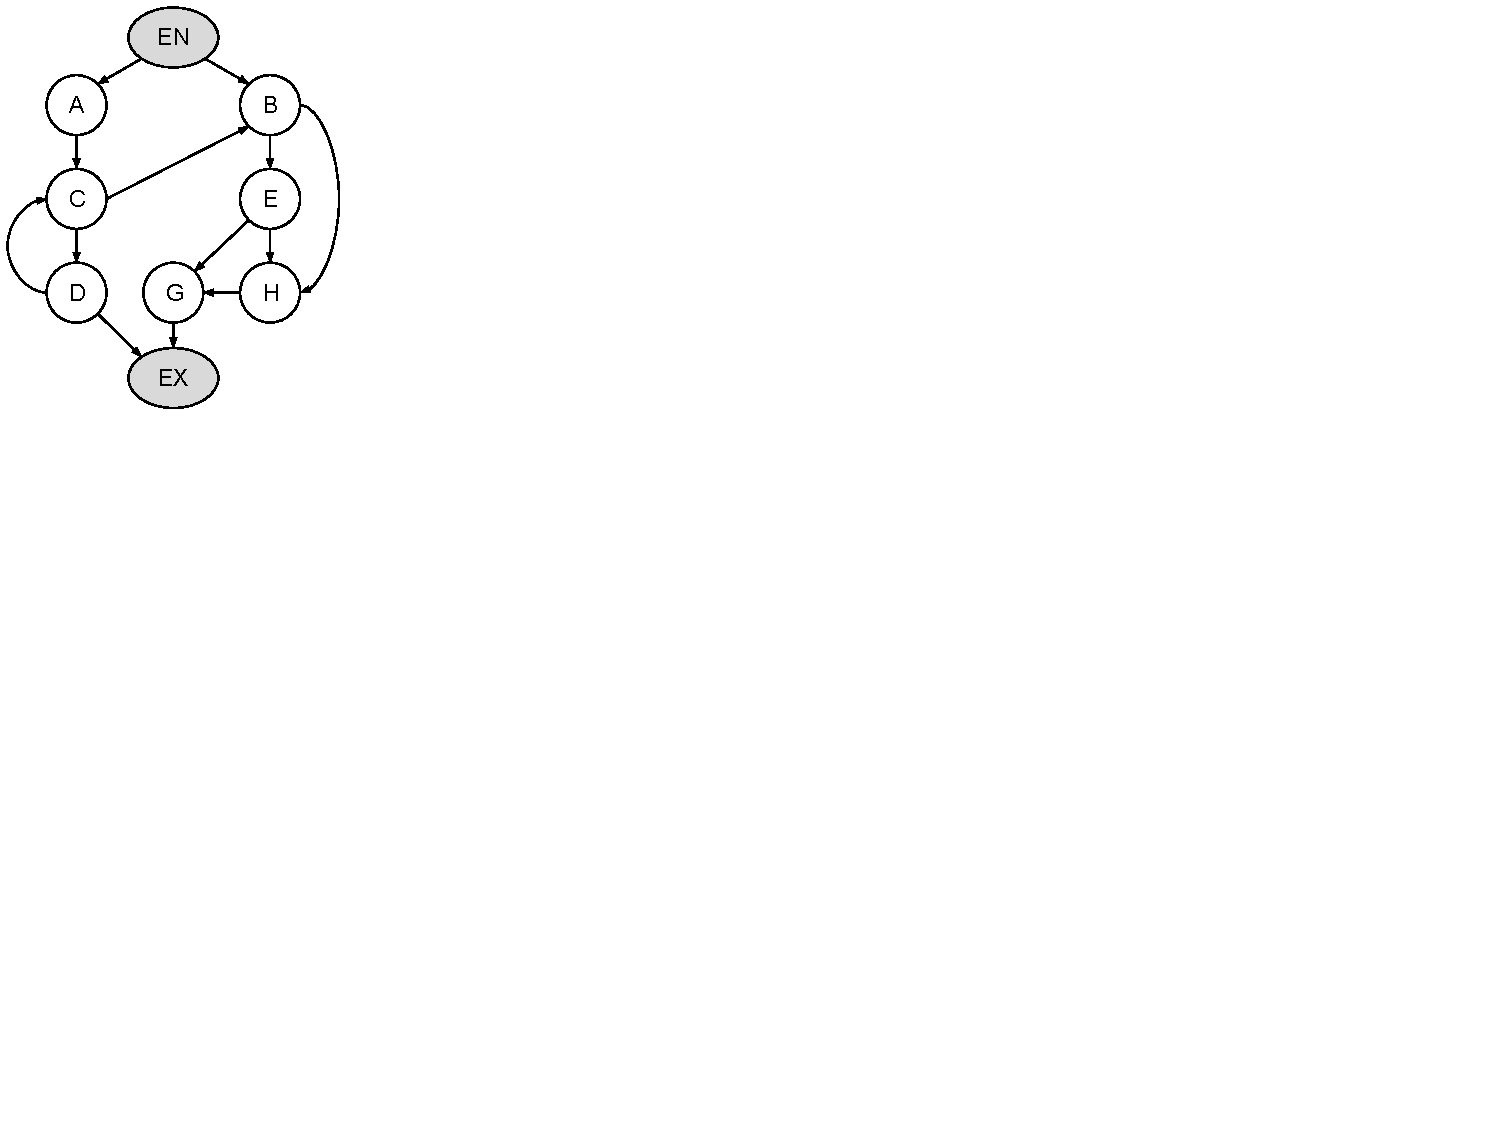
\includegraphics[clip, trim=0.1cm 12.1cm 19.6cm 0.1cm, width=\textwidth]{fig/bcov-03-probe-prunning}
        \caption{\small CFG}
        \label{fig:3:cfg}
    \end{subfigure}
    %    \hfill
    %    \begin{subfigure}[t]{0.19\textwidth}
    %        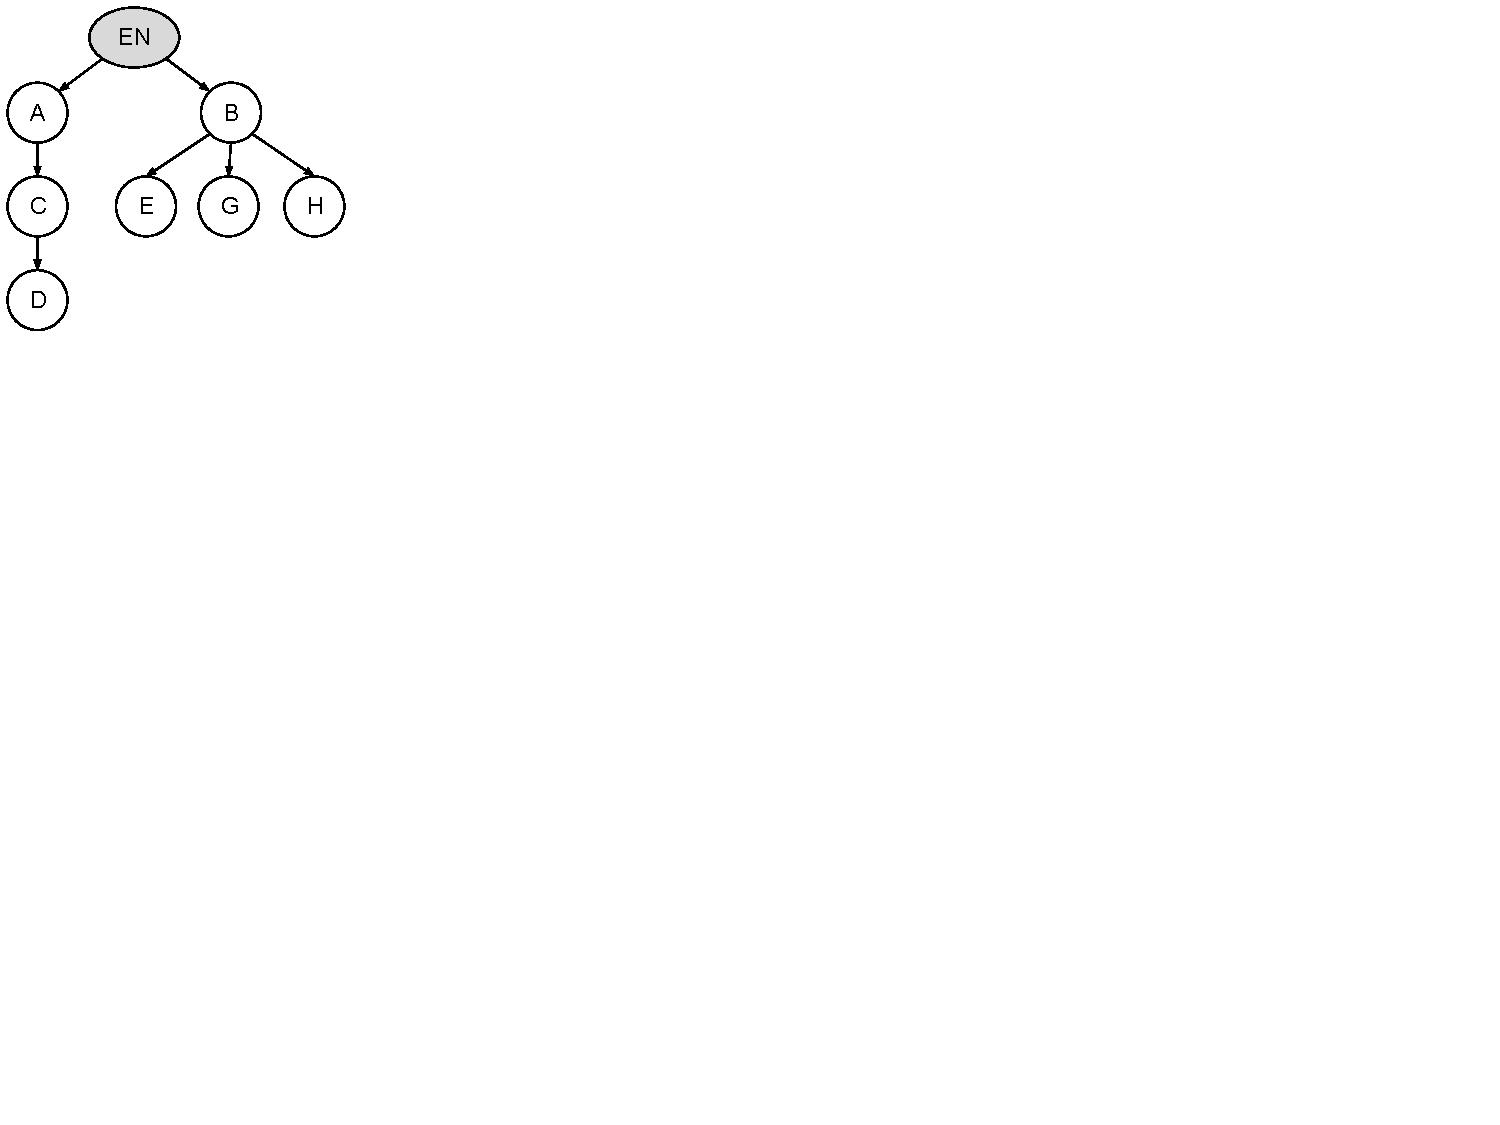
\includegraphics[clip, trim=0.1cm 12cm 19.5cm 0.1cm, width=\textwidth]{fig/bcov-03-predom}
    %        \caption{\small Predom tree}
    %        \label{fig:3:predom}
    %    \end{subfigure}
    %    \hfill
    %    \begin{subfigure}[t]{0.19\textwidth}
    %        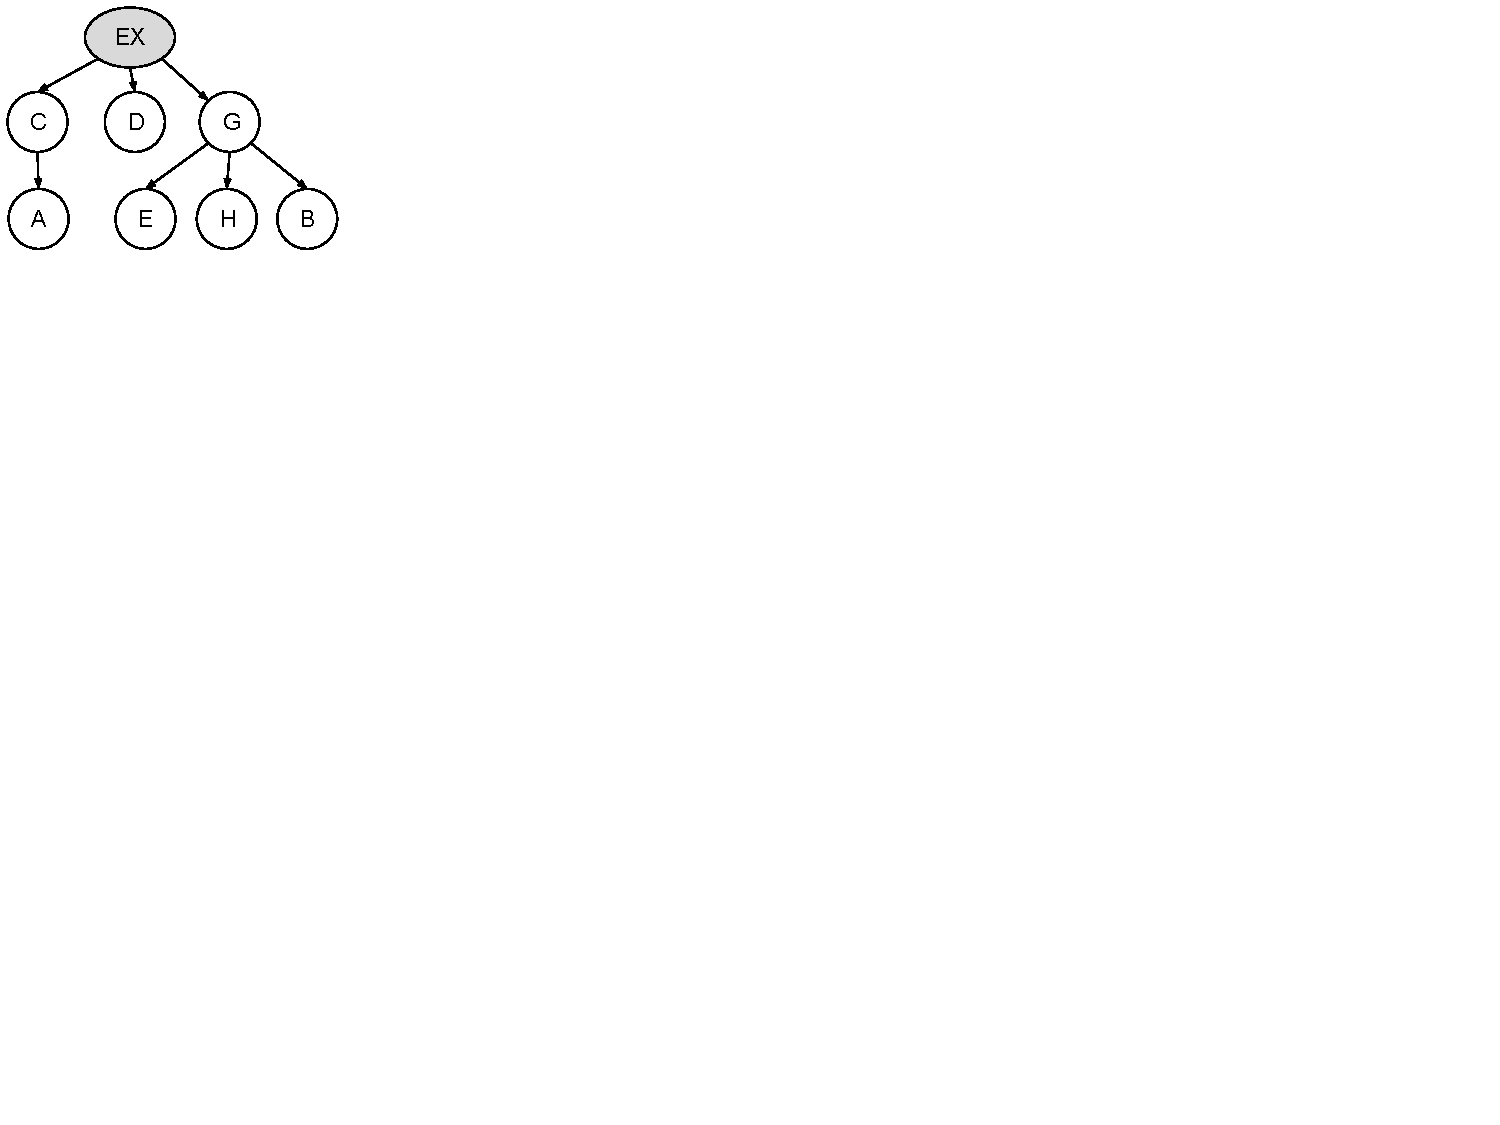
\includegraphics[clip, trim=0.1cm 12.2cm 19.6cm 0.1cm, width=\textwidth]{fig/bcov-03-postdom}
    %        \caption{\small Postdom tree}
    %        \label{fig:3:postdom}
    %    \end{subfigure}
    %    \hfill
    %    \begin{subfigure}[t]{0.185\textwidth}
    %        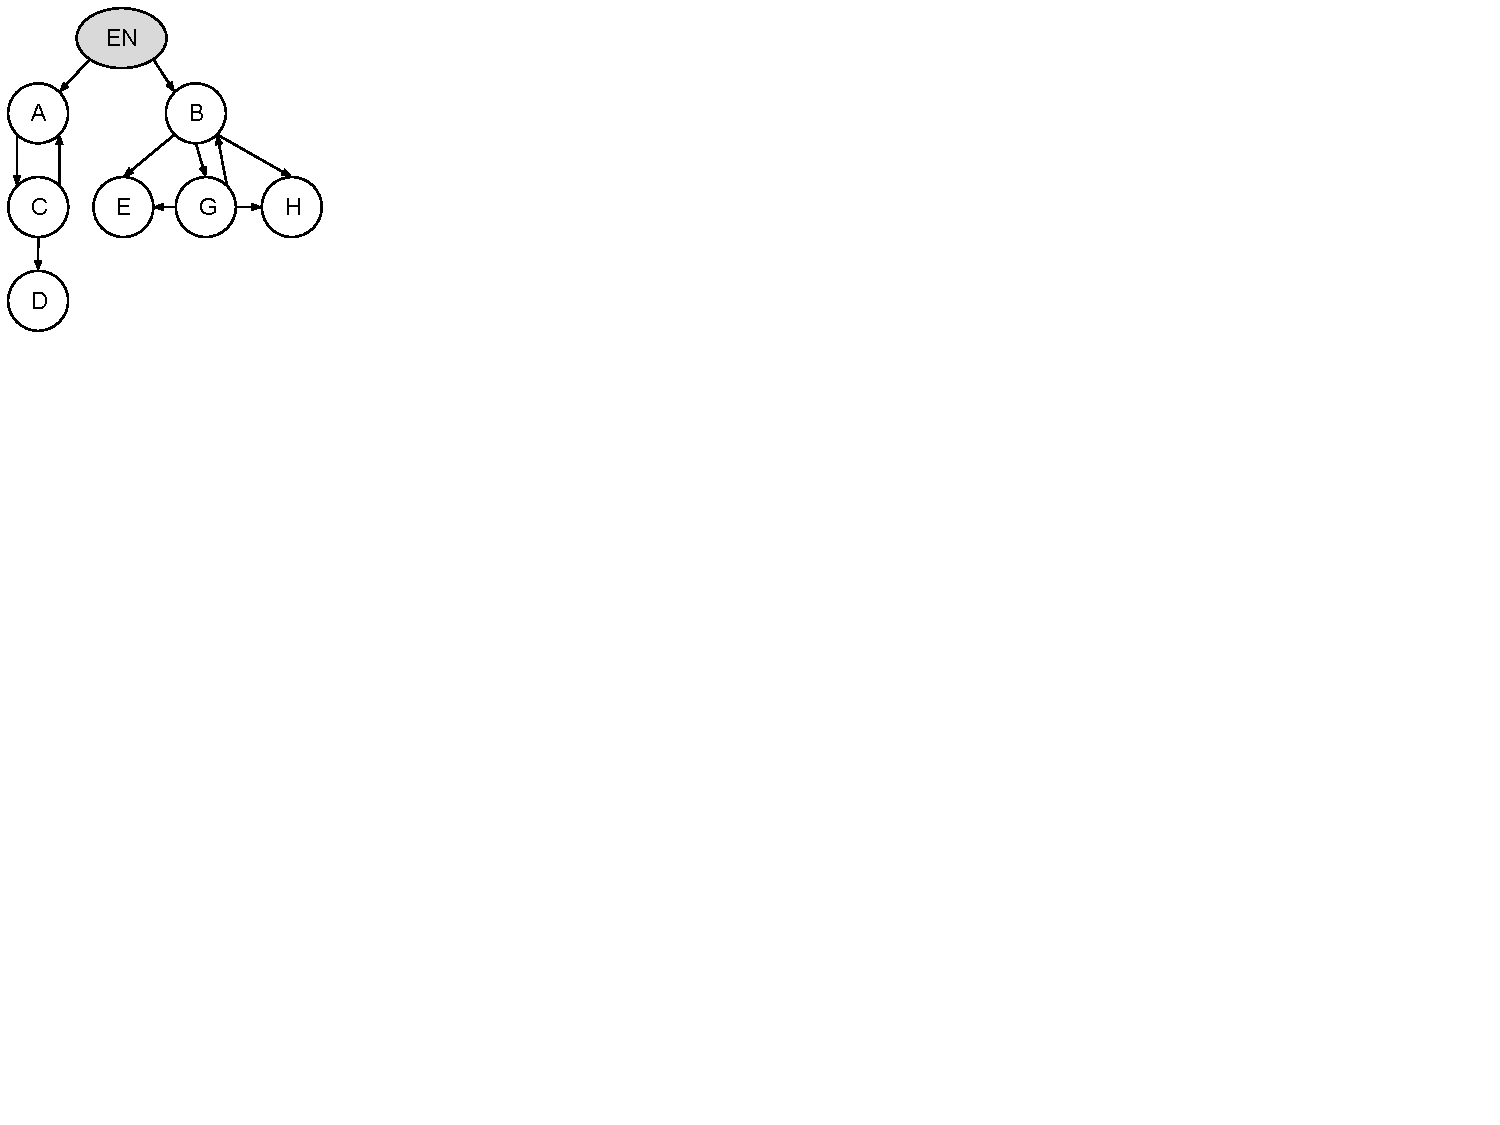
\includegraphics[clip, trim=0.1cm 12.4cm 19.9cm 0.1cm, width=\textwidth]{fig/bcov-03-domgraph}
    %        \caption{\small Dominator graph}
    %        \label{fig:3:domgraph}
    %    \end{subfigure}
    \hspace{0.5cm}
    \begin{subfigure}[t]{0.15\textwidth}
        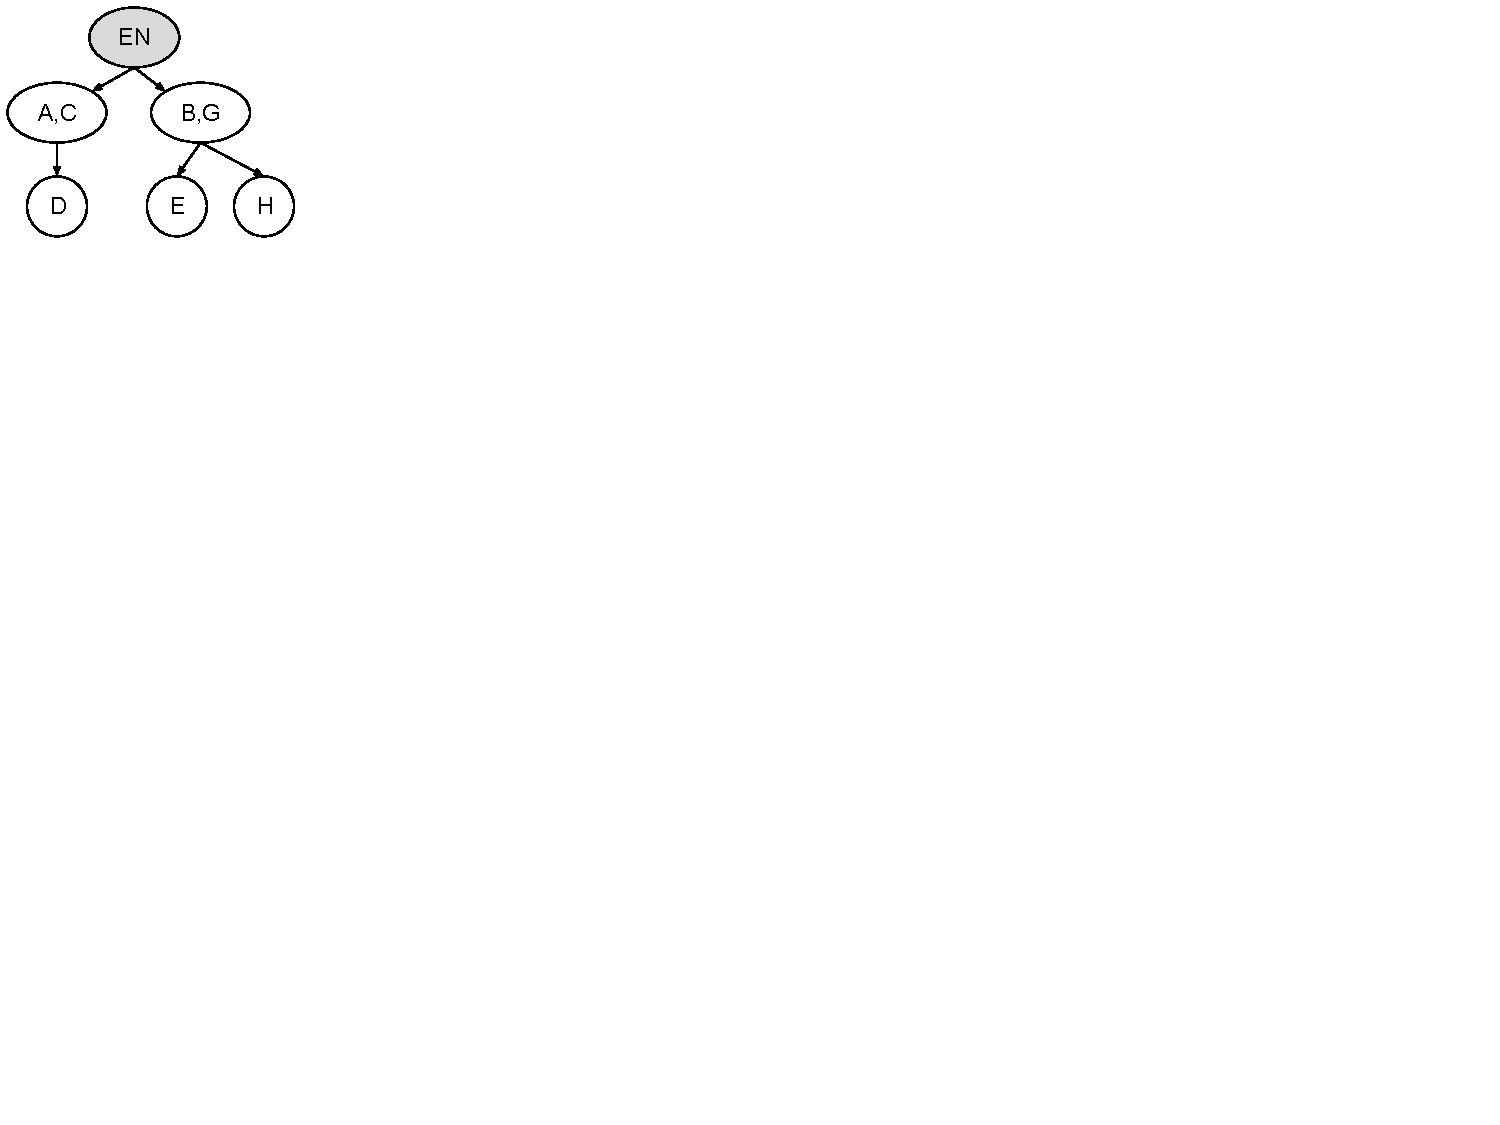
\includegraphics[clip, trim=0.1cm 12.6cm 20.4cm 0.1cm, width=\textwidth]{fig/bcov-03-sbgraph}
        
        \caption{\small SB-DG graph}
        \label{fig:3:sbgraph}
    \end{subfigure}
    
    \caption{An example CFG and its corresponding SB-DG.
        First, pre-domominator and post-dominator trees are constructed and merged in a dominator graph (DG). 
        SCCs in DG represent nodes in SB-DG.
        In the \textit{leaf-node} policy, only leaf nodes in SB-DG, namely, D, E, and H, need to be probed. 
        In the \textit{any-node} policy, either A or C need to be additionally probed.
        $EN$ and $EX$ are \textit{virtual} nodes commonly used to simplify dominance analysis.        
    }
    \Description{An example CFG and its corresponding SB-DG}
    \label{fig:probe-pruning}
\end{figure}

Generally, we are also interested in inferring the exact set of covered basic blocks given \textit{any} test input.
This is usually not possible in the leaf-node policy. 
For example, given an input that visits the path $A \rightarrow C \rightarrow B \rightarrow H \rightarrow G$, 
the leaf-node policy can report that the covered set is $\{B,H,G\}$. 
However, this policy can make no statement about the coverage of $A$ and $C$ since they do not dominate the visited probe in $H$.
We address this problem in the any-node policy.
The set of superblocks instrumented in this policy is a superset of those in the leaf-node policy.
More precisely, \mbox{$S_{any}=S_{leaf} \bigcup S_{c}$}.\linebreak
$S_c$ represents the set of \textit{critical} superblocks in the sense that each $sb \in S_c$ can be visited by at least one path in the CFG that does not visit any of its children in the SB-DG.

It is possible to determine $S_c$ using an $\mathcal{O}(|V|+|E|)$ algorithm where $V$ and $E$ are the nodes and edges in the CFG 
respectively.
We refer to \cite{Agrawal1994} for further details.
In Figure~\ref{fig:probe-pruning}, the superblock $\{B,G\}$ is non-critical. However, the superblock $\{A,C\}$ is critical and, consequently, will be probed in the any-node policy.

%%% Local Variables:
%%% mode: latex
%%% TeX-master: t
%%% End:
